\begin{frame}{}
	\begin{columns}[T]
		\begin{column}[c]{.25\textwidth}
			\centering
				\vspace{6\baselineskip}			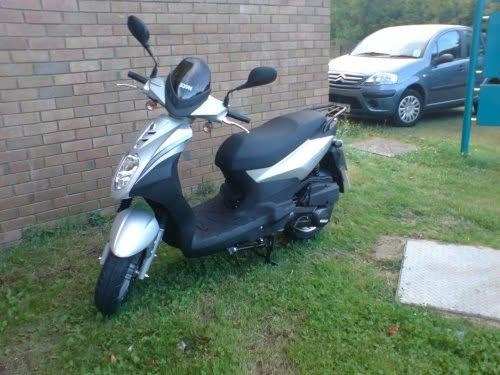
\includegraphics[width=\textwidth]{images/motorbike1.jpg}
		\end{column}
		
		\begin{column}[c]{.25\textwidth}
			\begin{figure}
				\centering
				\vspace{6\baselineskip}
				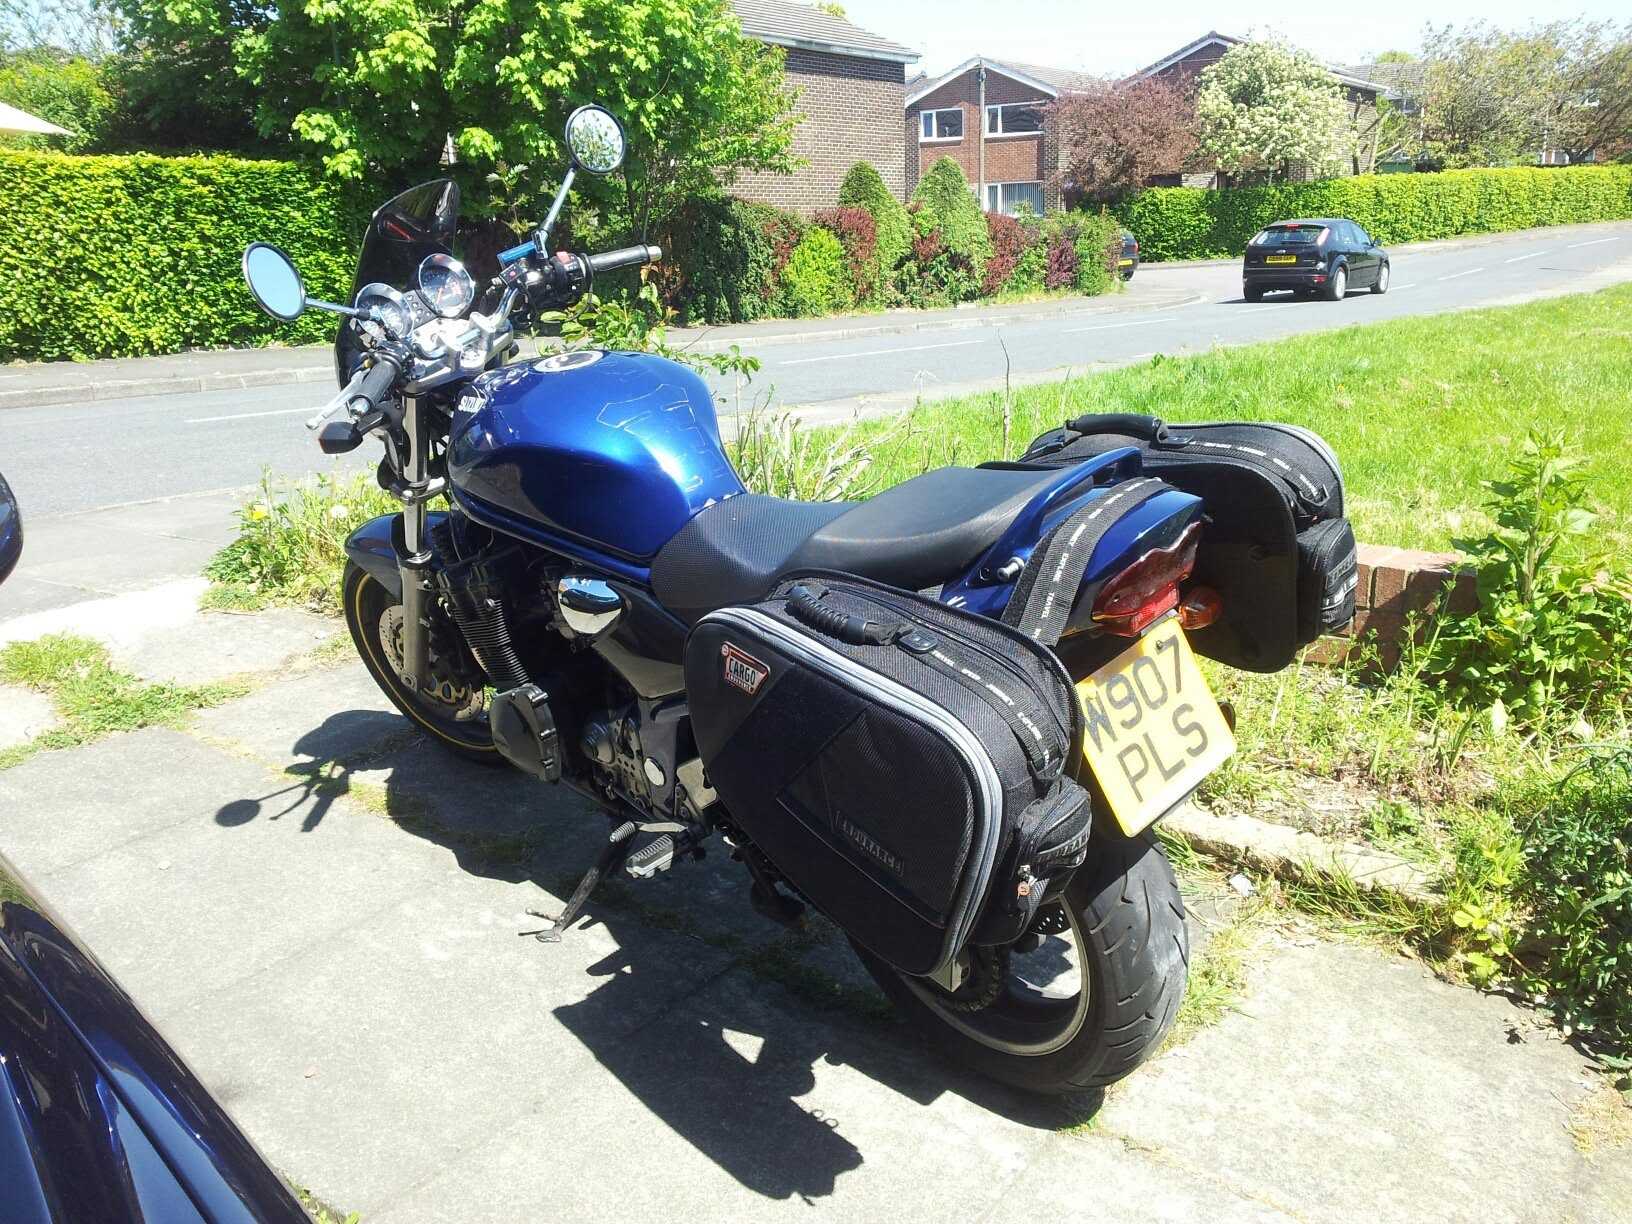
\includegraphics[width=\textwidth]{images/motorbike2.jpg}
			\end{figure}
		\end{column}
		
		\begin{column}[c]{.25\textwidth}
			\begin{figure}
				\centering
				\vspace{6\baselineskip}
				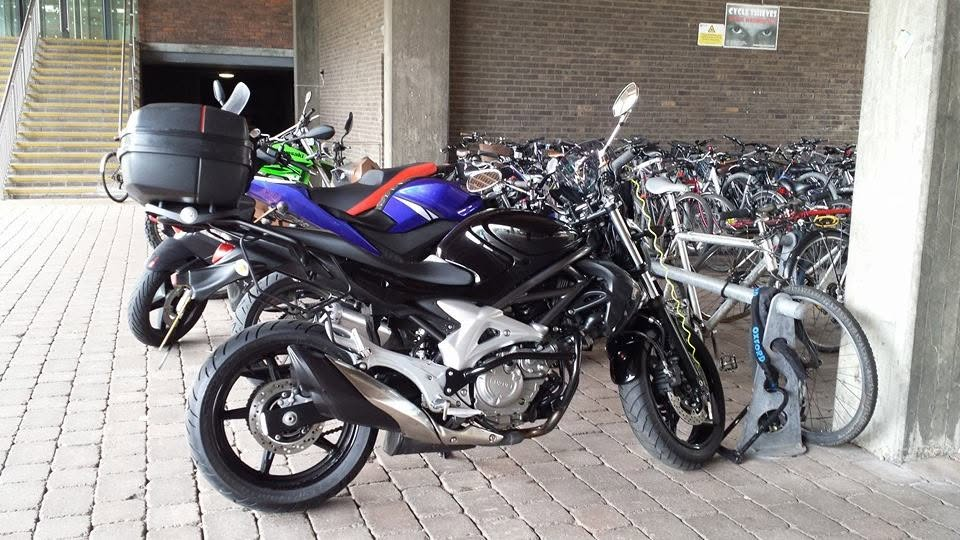
\includegraphics[width=\textwidth]{images/motorbike3.jpg}
			\end{figure}
		\end{column}
		
		\begin{column}[c]{.25\textwidth}
			\begin{figure}
				\centering
				\vspace{6\baselineskip}
				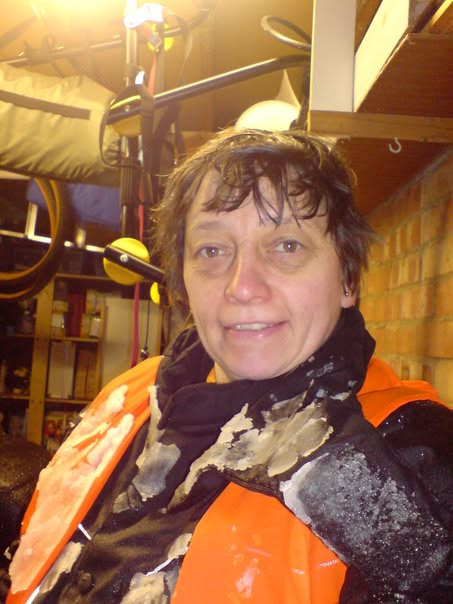
\includegraphics[width=\textwidth]{images/freezing.jpg}
			\end{figure}
		\end{column}
	\end{columns}
	\note{Step number 1. Get transport because as you might know, in England there are trains and buses - but that's it - they are there. You can really use them if you need to be somewhere within a certain timespan. They might or might not show up. As we used to say in South Africa: You can't complain about the service because there is no service to complain about.}
\end{frame}